\begin{itemize}
	\item Introduction to section(chapter)
	\item Why use vision as lozalization. cheap, no expensive sensors.
	\item About the MarkerLocator(out of scope), how it works,(Overview - not in depth, why it's slow, how window-mode works) how it's implemented, scalability.
	\item Quality meassure, why is it nessecary.
	\item How I arrived to a good way of meassureing the found marker.
	\item One drone detection
	\item Two drones detection, different ways of detecting orders.
	\item Implementation in ROS, splitting into different nodes.	optimization
\end{itemize}

\begin{figure}[H]
    \center
    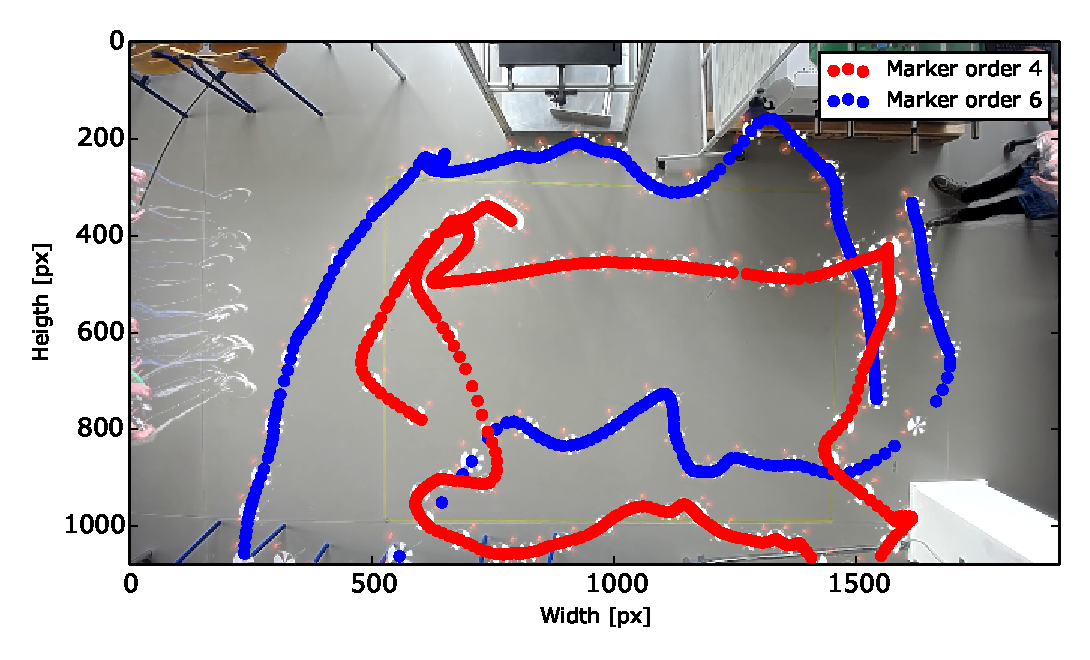
\includegraphics[width=1\textwidth]{graphics/test.eps}
  \label{fig:boat1}
  \caption{Figure showing every 7'th frame merged into one frame combined with the tracked positions of the drones}
\end{figure}
\Mathias{Smaller dot size - almost impossible to see the drone in the frames..}

\Mathias{Red is above blue, not because the drone wasn't detcted}
\Mathias{WIfi test distance, see what happens to latency}